% !TEX program = pdflatex
\documentclass[10pt]{report}

% ---------- PACKAGES ----------
\usepackage[margin=1in]{geometry}
\usepackage[T1]{fontenc}

\usepackage{setspace}
\usepackage{amsmath, amssymb}

\usepackage{xcolor}
\definecolor{softpink}{rgb}{0.99, 0.74, 0.71}

\usepackage{tikz}
\usetikzlibrary{shapes,patterns}

\usepackage{enumitem}

\usepackage{float}

\usepackage[hidelinks]{hyperref}
\usepackage{tocloft}
\usepackage{titlesec}

\setcounter{secnumdepth}{3}
\setcounter{tocdepth}{1}

\usepackage[most]{tcolorbox}
\usepackage[table]{xcolor}

% ---------- GRAPH SYSTEM (pgfplots) ----------
\usepackage{pgfplots}
\pgfplotsset{compat=1.18}

% ---------- BABY CANDY COLORS ----------
\definecolor{babyblue}{rgb}{0.68, 0.85, 0.90}
\definecolor{babypink}{rgb}{1.00, 0.80, 0.86}
\definecolor{babyyellow}{rgb}{1.00, 0.95, 0.70}
\definecolor{babyorange}{rgb}{1.00, 0.82, 0.65}
\definecolor{babygreen}{rgb}{0.75, 0.90, 0.75}

\setlength{\parindent}{0pt}
\setlength{\parskip}{0.35em}

\onehalfspacing

% ---------- HOMEWORK/TEST EXERCISE STYLING ----------
\newtcolorbox{hwbox}[1][]{
    colback=babyyellow!15,
    colframe=babyyellow!60!black,
    fonttitle=\bfseries,
    title={#1},
    breakable
}
\newtcolorbox{testbox}[1][]{
    colback=babygreen!15,
    colframe=babygreen!60!black,
    fonttitle=\bfseries,
    title={#1},
    breakable
}

% ---------- LISTINGS FOR R CODE ----------
\usepackage{listings}
\lstset{
    basicstyle=\ttfamily\small,
    backgroundcolor=\color{babyblue!10},
    frame=single,
    framerule=0.4pt,
    rulecolor=\color{babyblue!60!black},
    breaklines=true,
    showstringspaces=false,
    keywordstyle=\color{blue!70!black},
    commentstyle=\color{green!50!black},
    stringstyle=\color{red!60!black},
    language=R
}

\begin{document}

\begin{titlepage}
\centering
\vspace*{1cm}
{\LARGE MIE286 Lecture Notes After Midterm }\\[0.4cm]
{\large Probability and Statistics}\\[0.4cm]
{\large Cheryl Shi}\\[2cm]
\end{titlepage}

\tableofcontents
\newpage

% ============================================================
% PART 1: Fundamental Sampling Distributions and Data Descriptions
% ============================================================
\chapter{Chapter 8: Fundamental Sampling Distributions and Data Descriptions}

\section{Key Definitions}

\underline{Population}: The totality of observations with which we are concerned. In other words, it is the entire group of individuals or measurements of interest. We often cannot observe the entire population, so we rely on samples to make inferences.

\underline{Sample}: A subset of a population. We collect data on the sample and use it to draw conclusions about the population.

\underline{Parameter}: A number that describes the population. Parameters are fixed but in practice unknown. For example, the population mean $\mu$ and variance $\sigma^2$ are parameters. Since we rarely observe the whole population, we estimate parameters using statistics.

\underline{Statistic}: A function of sample data. It is itself a random variable with a distribution. For example, the sample mean $\bar{X}$ and sample variance $S^2$ are statistics. Because a statistic depends on which sample happens to be drawn, different samples produce different values of the statistic.

\textit{The key insight is that a statistic is a random variable. This means we can talk about its probability distribution, which leads to the concept of a sampling distribution.}

\section{Random Samples}

\begin{tcolorbox}[colback=softpink!15, colframe=softpink!60!black, title=Definition: Simple Random Sample]
The random variables $X_1, X_2, \ldots, X_n$ are said to form a \textbf{(simple) random sample} of size $n$ if the $X_i$'s are \textbf{i.i.d.}\ (independent, identically distributed), with each $X_i$ having probability distribution $f(x)$.
\end{tcolorbox}

Because the $X_i$ are independent and identically distributed, the joint distribution factors as:
\[
f(x_1, x_2, \ldots, x_n) = f(x_1)\,f(x_2)\cdots f(x_n).
\]

\textit{Why independence matters:} Independence means that the value of one observation does not affect the probability of any other observation. This is a reasonable assumption when the population is very large relative to the sample, or when sampling is done with replacement. In practice, even sampling without replacement from a large population is approximately independent.

\medskip

The sample mean is denoted $\bar{X}$ and computed as:
\[
\bar{X} = \frac{1}{n}\sum_{i=1}^n X_i.
\]

\textit{Conceptual picture:} Imagine taking many samples of size $n$ from the population. From each sample, compute $\bar{X}$. Each sample gives a different $\bar{X}$. The collection of all these sample means forms a distribution.

\begin{center}
\begin{tikzpicture}[scale=0.9]
  % Columns
  \node at (0, 4.5) {$X_1$};
  \node at (2, 4.5) {$X_{11}$};
  \node at (4, 4.5) {$X_{21}$};
  \node at (5.5, 4.5) {$\cdots$};

  \node at (0, 3.2) {$\vdots$};
  \node at (2, 3.2) {$\vdots$};
  \node at (4, 3.2) {$\vdots$};

  \node at (0, 2.0) {$X_n$};
  \node at (2, 2.0) {$X_{1n}$};
  \node at (4, 2.0) {$X_{2n}$};

  % Horizontal lines (sample averages)
  \draw[gray!60] (-0.7, 1.3) -- (5.0, 1.3);

  \node at (0, 0.7) {$\bar{X}$};
  \node at (2, 0.7) {$\bar{X}_1$};
  \node at (4, 0.7) {$\bar{X}_2$};

  % Right column labels
  \node[right] at (7, 4.5) {$X_1 \sim f(x)$};
  \node[right] at (7, 2.0) {$X_n \sim f(x)$};
  \node[right] at (7, 0.7) {$\bar{X}$ is a r.v.\ $\longrightarrow$ Sampling Distribution};
\end{tikzpicture}
\end{center}

Each column represents a separate sample drawn from the same population. The bottom row shows the sample mean computed for each sample. The distribution of all these sample means is the \textit{sampling distribution} of $\bar{X}$.

\section{Sampling Distribution}

\begin{tcolorbox}[colback=babyblue!15, colframe=babyblue!60!black, title=Definition: Sampling Distribution]
The probability distribution of a statistic is called a \textbf{sampling distribution}. It describes the variability of the statistic across all possible samples of the same size from the same population.
\end{tcolorbox}

The sampling distribution depends on:
\begin{itemize}
  \item the size of the population,
  \item the size of the sample, and
  \item the method of sampling.
\end{itemize}

\textit{Why sampling distributions matter:} The sampling distribution tells us how much a statistic (like $\bar{X}$) would vary from sample to sample. This is the foundation for making inferences about population parameters---it allows us to quantify uncertainty.

\section{Sampling from a Normal Distribution}

\subsection{Theorem: Distribution of the Sample Mean from a Normal Population}

\begin{tcolorbox}[colback=softpink!15, colframe=softpink!60!black, title=Theorem (Normal Population)]
Suppose a random sample of size $n$ is taken from $N(\mu, \sigma^2)$. That is,
\[
X_1, X_2, \ldots, X_n \overset{\text{iid}}{\sim} N(\mu,\,\sigma^2).
\]
Each observation $X_i$, $i = 1, 2, \ldots, n$, has the same distribution. Then:
\[
\bar{X} \sim N\!\left(\mu,\;\frac{\sigma^2}{n}\right)
\]
and equivalently,
\[
\sum_{i=1}^n X_i \sim N(n\mu,\; n\sigma^2).
\]
\end{tcolorbox}

\textit{This was shown through moment generating functions (mgf's).} Recall that the mgf of $N(\mu, \sigma^2)$ is $M_X(t) = \exp\!\left(\mu t + \frac{1}{2}\sigma^2 t^2\right)$.

\medskip

\textbf{Proof (via mgf's):}

The mgf of a single $X_i \sim N(\mu, \sigma^2)$ is:
\[
M_{X_i}(t) = \exp\!\left(\mu t + \tfrac{1}{2}\sigma^2 t^2\right).
\]

For the sum $\sum_{i=1}^n X_i$, since the $X_i$ are independent:
\[
M_{\sum X_i}(t) = \prod_{i=1}^n M_{X_i}(t) = \left[\exp\!\left(\mu t + \tfrac{1}{2}\sigma^2 t^2\right)\right]^n = \exp\!\left(n\mu t + \tfrac{1}{2}\,n\sigma^2 t^2\right).
\]

This is the mgf of $N(n\mu,\; n\sigma^2)$, so $\sum_{i=1}^n X_i \sim N(n\mu,\; n\sigma^2)$.

For the sample mean $\bar{X} = \frac{1}{n}\sum X_i$, we use $M_{\bar{X}}(t) = M_{\sum X_i}(t/n)$:
\[
M_{\bar{X}}(t) = \exp\!\left(n\mu\cdot\frac{t}{n} + \frac{1}{2}\,n\sigma^2\cdot\frac{t^2}{n^2}\right) = \exp\!\left(\mu t + \frac{1}{2}\cdot\frac{\sigma^2}{n}\cdot t^2\right).
\]

This is the mgf of $N\!\left(\mu, \frac{\sigma^2}{n}\right)$. Therefore $\bar{X} \sim N\!\left(\mu, \frac{\sigma^2}{n}\right)$. \hfill $\square$

\medskip

\textit{Key takeaway:} The sample mean $\bar{X}$ is centered at the true population mean $\mu$. Its variance $\sigma^2/n$ shrinks as $n$ grows, meaning larger samples produce more precise estimates of $\mu$.

\section{The Central Limit Theorem (CLT)}

The previous result required the population to be normal. The Central Limit Theorem is a much more powerful result that applies to \emph{any} distribution.

\begin{tcolorbox}[colback=babyblue!15, colframe=babyblue!60!black, title=Central Limit Theorem]
Let $X_1, X_2, \ldots, X_n$ be independent random variables from the \emph{same} distribution with mean $\mu$ and variance $\sigma^2$. Then the limiting form of the distribution of
\[
Z = \frac{\bar{X} - \mu}{\sigma / \sqrt{n}},
\]
as $n \to \infty$, is the standard normal distribution.
\end{tcolorbox}

\textbf{Rule of thumb:} The approximation is generally considered adequate when $n \geq 30$.

\medskip

\textit{Why this is powerful:} Even if the individual $X_i$ follow a skewed, uniform, exponential, or other non-normal distribution, once we average enough of them together, the distribution of the average becomes approximately normal. This is the theoretical foundation for much of classical statistics.

\medskip

\textbf{Equivalent formulations of the CLT:}

\begin{enumerate}
  \item If $X_i$ are i.i.d.\ from a distribution with mean $\mu$ and variance $\sigma^2$, then:
  \[
  \bar{X} \;\overset{\text{approx}}{\sim}\; N\!\left(\mu,\;\frac{\sigma^2}{n}\right) \qquad \text{for large } n.
  \]
  
  \item For the sum: if $\bar{X} \overset{\text{approx}}{\sim} N\!\left(\mu, \frac{\sigma^2}{n}\right)$, then:
  \[
  \sum_{i=1}^n X_i \;\overset{\text{approx}}{\sim}\; N(n\mu,\; n\sigma^2).
  \]
\end{enumerate}

\textit{Remark:} $n \geq 30$ is a good cutoff for the approximation. For populations that are already close to normal, the CLT kicks in for much smaller $n$. For highly skewed populations, you may need larger $n$.

\section{Data Descriptions: Quantiles, Boxplots, and QQ-Plots}

\subsection{Quantiles}

A \underline{quantile} of a sample (say $x_p$) is the value below which a specific fraction $p$ of the data values fall. Quantiles are often described as \textbf{percentiles}.

\textbf{Quartiles} are special cases of quantiles:
\begin{itemize}
  \item 1st quartile $Q_1$ (25th percentile),
  \item 2nd quartile $Q_2$ (50th percentile, i.e., the median),
  \item 3rd quartile $Q_3$ (75th percentile).
\end{itemize}

The \textbf{five-number summary} of a dataset consists of: $\min, \; Q_1, \; Q_2, \; Q_3, \; \max$.

\subsection{Boxplot}

A boxplot is a graphical display based on the five-number summary. It shows:
\begin{itemize}
  \item a box from $Q_1$ to $Q_3$ (the \textbf{interquartile range}, IQR $= Q_3 - Q_1$),
  \item a line at the median inside the box,
  \item whiskers extending to the smallest and largest observations within $1.5 \times \text{IQR}$ of the quartiles,
  \item individual points (possible outliers) beyond the whiskers.
\end{itemize}

\begin{center}
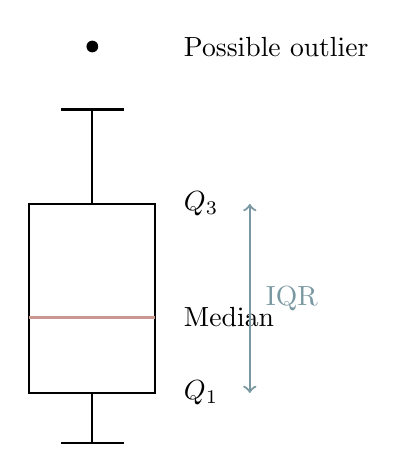
\begin{tikzpicture}[scale=0.8]
  % Box
  \draw[thick] (2, 0) rectangle (4, 3);
  % Median line
  \draw[very thick, softpink!80!black] (2, 1.2) -- (4, 1.2);
  % Whiskers
  \draw[thick] (3, 3) -- (3, 4.5);
  \draw[thick] (2.5, 4.5) -- (3.5, 4.5);
  \draw[thick] (3, 0) -- (3, -0.8);
  \draw[thick] (2.5, -0.8) -- (3.5, -0.8);
  % Outlier
  \node[fill=black, circle, inner sep=1.5pt] at (3, 5.5) {};
  % Labels
  \node[right] at (4.3, 3) {$Q_3$};
  \node[right] at (4.3, 1.2) {Median};
  \node[right] at (4.3, 0) {$Q_1$};
  \node[right] at (4.3, 5.5) {Possible outlier};
  \draw[<->, thick, babyblue!70!black] (5.5, 0) -- (5.5, 3);
  \node[right, babyblue!70!black] at (5.6, 1.5) {IQR};
\end{tikzpicture}
\end{center}

\subsection{Quantile Plot}

A \underline{quantile plot} displays data values on the vertical axis against the fraction of observations exceeded by the data value on the horizontal axis. Key properties:
\begin{itemize}
  \item All data points are plotted (unlike a boxplot which summarizes).
  \item It is \textbf{descriptive}, not diagnostic.
\end{itemize}

\subsection{Normal Quantile-Quantile (QQ) Plot}

The normal QQ-plot is a \textbf{diagnostic} tool used to determine whether a data set came from a normal distribution.

\begin{itemize}
  \item Plot the data quantiles (vertical axis) against the corresponding quantiles of the standard normal distribution (horizontal axis).
  \item If the data are approximately normal, the points will fall approximately on a \textbf{straight line}.
  \item Systematic deviations from linearity indicate non-normality.
  \item \textbf{Outliers} appear as points that are far from the overall pattern.
\end{itemize}

\textit{Note on the textbook:} The x-axis labels in the book's QQ-plot figure should be $-2, -1, 0, 1, 2$ (standard normal quantiles), not the values shown.

\subsection{Normal Probability Plot}

Similar to the QQ-plot, but rather than corresponding $z$-scores we have corresponding standard normal percentiles and a special scale. The interpretation is the same:
\begin{itemize}
  \item Look for a straight line --- systematic deviations indicate non-normality.
  \item Outliers appear as points far from the overall pattern.
\end{itemize}

\section{Chebyshev's Inequality}

\begin{tcolorbox}[colback=softpink!15, colframe=softpink!60!black, title=Theorem: Chebyshev's Inequality]
The probability that $X$ will assume a value within $k$ standard deviations of the mean is at least $1 - \frac{1}{k^2}$:
\[
P\!\left(\mu - k\sigma < X < \mu + k\sigma\right) \geq 1 - \frac{1}{k^2}.
\]
\end{tcolorbox}

\textit{Interpretation:} Chebyshev's inequality gives a lower bound on probability that works for \textbf{any} distribution (as long as the mean and variance exist). It does not require normality.

\medskip

\textbf{Proof (continuous case):}

We start with the definition of variance:
\[
\sigma^2 = \int_{-\infty}^{\infty} (x - \mu)^2 f(x)\,dx.
\]

Split the integral into three regions:
\[
\sigma^2 = \int_{-\infty}^{\mu - k\sigma} (x-\mu)^2 f(x)\,dx + \int_{\mu-k\sigma}^{\mu+k\sigma} (x-\mu)^2 f(x)\,dx + \int_{\mu+k\sigma}^{\infty} (x-\mu)^2 f(x)\,dx.
\]

Since the middle integral is non-negative, we can drop it to get a lower bound:
\[
\sigma^2 \geq \int_{-\infty}^{\mu - k\sigma} (x-\mu)^2 f(x)\,dx + \int_{\mu+k\sigma}^{\infty} (x-\mu)^2 f(x)\,dx.
\]

For $x \leq \mu - k\sigma$ or $x \geq \mu + k\sigma$, we have $|x - \mu| \geq k\sigma$, so $(x - \mu)^2 \geq k^2\sigma^2$. Substituting:
\[
\sigma^2 \geq k^2\sigma^2 \left[\int_{-\infty}^{\mu - k\sigma} f(x)\,dx + \int_{\mu+k\sigma}^{\infty} f(x)\,dx\right].
\]

Dividing both sides by $k^2\sigma^2$:
\[
\int_{-\infty}^{\mu - k\sigma} f(x)\,dx + \int_{\mu+k\sigma}^{\infty} f(x)\,dx \leq \frac{1}{k^2}.
\]

Therefore:
\[
P\!\left(\mu - k\sigma < X < \mu + k\sigma\right) = 1 - \left[\int_{-\infty}^{\mu-k\sigma} f(x)\,dx + \int_{\mu+k\sigma}^{\infty} f(x)\,dx\right] \geq 1 - \frac{1}{k^2}. \qquad \square
\]

\section{R Code: QQ-Plots and CLT Demonstration}

\subsection{Creating Random Samples and QQ-Plots}

\begin{lstlisting}
# Creating random samples from a given distribution
x <- rf(2000, 3, 27)       # random sample of size 2000 from F(3, 27)
x <- rnorm(100, 2, 100)    # random sample of size 100 from N(2, 100)

# Plotting a normal quantile-quantile plot
qqnorm(x)
qqline(x)

# For the normal probability plot (requires "e1071" package)
library(e1071)
probplot(x)    # draw a normal probability plot
\end{lstlisting}

\subsection{Demonstrating the CLT}

The idea is to:
\begin{enumerate}
  \item Generate random data from a non-normal distribution (e.g., $F(3, 27)$, which is right-skewed).
  \item Repeatedly draw samples of size $n$ and compute the sample mean each time.
  \item Plot the distribution of these sample means.
  \item Observe that as $n$ increases, the distribution of $\bar{X}$ becomes more and more normal.
\end{enumerate}

\begin{lstlisting}
# Show that the F(3,27) distribution is right-skewed
x <- rf(2000, 3, 27)
hist(x)

# CLT demonstration
n <- 4    # try different values: n=4, 10, 30, 100
xbar <- array(0, dim = c(0, 1000))  # vector of 1000 zeros

for(i in 1:1000) {
  xbar[i] <- mean(rf(n, 3, 27))     # sample mean of n obs from F(3,27)
}

hist(xbar)       # should look more normal as n increases
qqnorm(xbar)     # should fall on a straight line
qqline(xbar)
\end{lstlisting}

\textit{Key observation:} When $n = 4$, the histogram of $\bar{X}$ is still somewhat skewed. As $n$ increases to 30 or more, the histogram looks approximately normal and the QQ-plot becomes nearly linear. This is the Central Limit Theorem in action.

\section{True or False: Conceptual Questions}

The following true/false questions test understanding of sampling distributions and the CLT:

\begin{enumerate}
  \item \textbf{As $n$ (sample size) increases, the mean of the sampling distribution of $\bar{X}$ decreases.}
  
  \textit{False.} The mean of $\bar{X}$ is always $\mu$, regardless of $n$. The sample size does not affect the center of the sampling distribution.
  
  \item \textbf{As $n$ increases, the standard deviation of the sampling distribution of $\bar{X}$ decreases.}
  
  \textit{True.} The standard deviation of $\bar{X}$ is $\sigma/\sqrt{n}$, which decreases as $n$ grows. Larger samples produce more precise estimates.
  
  \item \textbf{The mean $\bar{X}$ of a random sample of size 4 from a left-skewed distribution is approximately normally distributed.}
  
  \textit{False.} The CLT requires $n \geq 30$ (approximately) for the normal approximation to be adequate. With $n = 4$ from a skewed distribution, $\bar{X}$ will not be approximately normal.
  
  \item \textbf{The distribution of the proportion of successes $\hat{p}$ in a sufficiently large sample is approximately normal with mean $p$ and std.\ dev.\ $\sqrt{np(1-p)}$.}
  
  \textit{False.} The standard deviation of $\hat{p} = X/n$ is $\sqrt{p(1-p)/n}$, not $\sqrt{np(1-p)}$. The quantity $\sqrt{np(1-p)}$ is the standard deviation of the \textit{count} $X$, not the proportion $\hat{p}$.
  
  \item \textbf{If $\bar{X}$ is the mean of a simple random sample of size 9 from $N(500, \sigma^2 = 18)$, then $\bar{X}$ has a normal distribution with mean 500 and variance 36.}
  
  \textit{False.} Since $X_i \sim N(500, 18)$, we have $\bar{X} \sim N(500, 18/9) = N(500, 2)$. The variance of $\bar{X}$ is $18/9 = 2$, not 36.
  
  \item \textbf{A large sample from a skewed population distribution will have an approximately normal histogram.}
  
  \textit{False.} The \textit{data itself} will still look skewed. It is the \textit{sampling distribution of $\bar{X}$} that becomes approximately normal, not the distribution of the raw data.
  
  \item \textbf{The mean of a population will be normally distributed if the population is quite large.}
  
  \textit{False.} The population mean $\mu$ is a fixed number (a parameter), not a random variable. It does not have a distribution. The CLT applies to the \textit{sample mean} $\bar{X}$, not to the population mean.
  
  \item \textbf{The average blood cholesterol level recorded in a simple random sample of 100 students from a large population will be approximately normally distributed.}
  
  \textit{True.} By the CLT, with $n = 100 \geq 30$, the sample mean $\bar{X}$ is approximately normal regardless of the shape of the population distribution.
\end{enumerate}

\bigskip

% ============================================================
% PART 2: Sampling Distributions and Inferences on the Population Mean
% ============================================================

\section{Examples: Applying the CLT to the Sum of Random Variables}

\subsection{Example 1: Airline Passenger Weights}

\textbf{Problem.} Weights of airline passengers are known to have a distribution with mean $\mu = 75\,\text{kg}$ and standard deviation $\sigma = 10\,\text{kg}$. A certain plane has a passenger weight capacity of $7700\,\text{kg}$. What is the probability that a flight of 100 passengers will exceed the capacity?

\textbf{Setup.} Let $X_i$ denote the weight (in kg) of the $i$-th passenger, so $X_i \sim (\mu = 75, \sigma = 10)$. Since passengers are randomly selected, $X_1, \ldots, X_{100}$ are i.i.d. We want:
\[
P\!\left(\sum_{i=1}^{100} X_i > 7700\right).
\]

\textbf{Intuition.} If each passenger weighs 75 kg on average, then 100 passengers should total around $100 \times 75 = 7500\,\text{kg}$. The question is how likely the total exceeds 7700 kg.

\textbf{Solution.} By the CLT (since $n = 100 \geq 30$):
\[
\sum_{i=1}^{100} X_i \;\overset{\text{approx}}{\sim}\; N\!\left(100 \times 75,\; 100 \times 100\right) = N\!\left(7500,\; 10000\right).
\]
The variance of the sum is $n\sigma^2 = 100 \times 10^2 = 10{,}000$, so the standard deviation is $\sqrt{10{,}000} = 100$.

\[
P\!\left(\sum_{i=1}^{100} X_i > 7700\right) = P\!\left(Z > \frac{7700 - 7500}{\sqrt{100 \times 100}}\right) = P\!\left(Z > \frac{200}{100}\right) = P(Z > 2) \approx \boxed{0.0228.}
\]

\textit{Conclusion:} There is approximately a 2.28\% chance the flight exceeds the weight capacity.

\bigskip

% ============================================================
\section{Inferences on the Population Mean}
% ============================================================

So far, we have used probability to compute things given known parameters (e.g., ``given $\mu = 75$, find $P(\ldots)$''). Now we flip the question: given observed data, what can we infer about the unknown $\mu$?

\subsection{The Setup}

We have a sample $X_1, \ldots, X_n$ that are i.i.d.\ with unknown mean $\mu$ and known (or estimable) standard deviation $\sigma$. We observe the sample mean $\bar{X}$ and ask: is the data consistent with a particular assumed value of $\mu$?

By the CLT (when $n$ is large), we know:
\[
\bar{X} \sim N\!\left(\mu, \frac{\sigma^2}{n}\right).
\]

\subsection{Example 2: Cylindrical Component Diameters}

\textbf{Problem.} A manufacturing process produces cylindrical components. An engineer conjectures that the population mean diameter is $\mu = 5\,\text{mm}$. A random sample of $n = 100$ parts is selected, yielding $\bar{x} = 5.027\,\text{mm}$. It is known that $\sigma = 0.1\,\text{mm}$. Does the sample support the engineer's conjecture?

\textit{Note:} In practice, $\sigma$ is rarely ``known'' exactly. Here we take it as a given assumption --- perhaps it was established from extensive prior production data. The case where $\sigma$ must be estimated from the sample leads to $t$-procedures covered later.

\textbf{Setup.} Let $X_i$ be the diameter of the $i$-th component (in mm). Then $X_1, \ldots, X_{100}$ are i.i.d.\ with unknown $\mu$ and $\sigma = 0.1$. By the CLT:
\[
\bar{X} \sim N\!\left(\mu, \;\frac{0.1^2}{100}\right) = N\!\left(\mu,\; \frac{0.01}{100}\right).
\]
The standard deviation of $\bar{X}$ is $\dfrac{0.1}{\sqrt{100}} = 0.01$.

\textbf{Assuming $\mu = 5$.} How unlikely is it to observe a sample mean that deviates from 5 by 0.027 mm or more?

\[
P\!\left(\bar{X} \leq 4.973 \;\text{ or }\; \bar{X} \geq 5.027 \;\Big|\; \mu = 5\right) = 1 - P(4.973 < \bar{X} < 5.027)
\]

By symmetry:
\[
= 2\,P\!\left(Z > \frac{5.027 - 5}{0.1/10}\right) = 2\,P\!\left(Z > \frac{0.027}{0.01}\right) = 2\,P(Z > 2.7) \approx \boxed{0.007.}
\]

\textbf{Visualization.} The sampling distribution of $\bar{X}$ under $\mu = 5$ is shown below. The shaded tails represent the probability of observing a sample mean as extreme as or more extreme than $\bar{x} = 5.027$.

\begin{center}
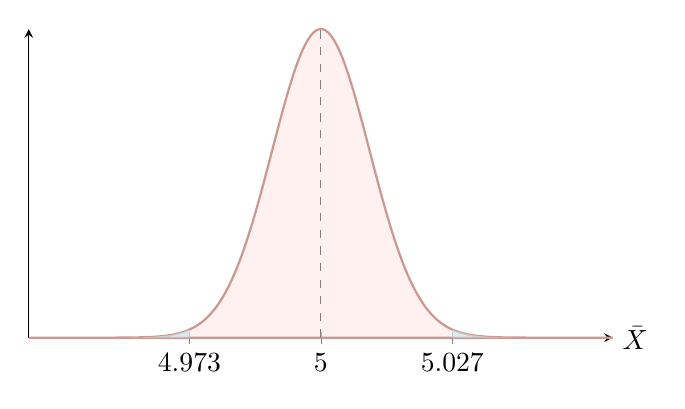
\begin{tikzpicture}
\begin{axis}[
  width=9cm, height=5.5cm,
  domain=4.94:5.06,
  samples=200,
  axis lines=left,
  xlabel={$\bar{X}$},
  ylabel={},
  xtick={4.973, 5, 5.027},
  xticklabels={4.973, 5, 5.027},
  ytick=\empty,
  every axis x label/.style={at={(axis cs:5.06,0)}, anchor=west},
  clip=false
]
  % Normal curve centered at 5 with std dev 0.01
  \addplot[thick, softpink!80!black, fill=softpink!40, fill opacity=0.5]
    {exp(-((x-5)^2)/(2*0.01^2)) / (0.01*sqrt(2*pi))}
    \closedcycle;
  % Shade left tail
  \addplot[fill=babyblue!60, fill opacity=0.7, draw=none, domain=4.94:4.973, samples=50]
    {exp(-((x-5)^2)/(2*0.01^2)) / (0.01*sqrt(2*pi))} \closedcycle;
  % Shade right tail
  \addplot[fill=babyblue!60, fill opacity=0.7, draw=none, domain=5.027:5.06, samples=50]
    {exp(-((x-5)^2)/(2*0.01^2)) / (0.01*sqrt(2*pi))} \closedcycle;
  % Vertical line at center
  \draw[dashed, gray] (axis cs:5, 0) -- (axis cs:5, 40);
\end{axis}
\end{tikzpicture}
\end{center}

\textbf{Interpretation.} A probability of $0.007 = 0.7\%$ means that, \emph{if the true mean really were 5 mm}, observing a sample mean as far as 5.027 mm from 5 would be a very rare event. Since 0.007 is well below the conventional threshold of $\alpha = 0.05$, we say the observed data \textbf{does NOT support} the engineer's conjecture that $\mu = 5\,\text{mm}$.

\medskip

\textit{On the significance threshold $\alpha = 0.05$:} In science and engineering, the conventional cutoff for declaring a result statistically significant is $\alpha = 0.05$ (5\%). This is sometimes called the ``risk bound'' or significance level. If the probability of seeing data at least as extreme as what we observed---assuming the null hypothesis is true---falls below $\alpha$, we reject the null hypothesis. Here, $0.007 < 0.05$, so we reject $\mu = 5$.

\bigskip

% ============================================================
\section{Sampling Distribution of the Difference Between Two Averages}
% ============================================================

\begin{tcolorbox}[colback=softpink!15, colframe=softpink!60!black, title=Theorem: Two-Sample Difference of Means]
Let independent random samples of sizes $n_1$ and $n_2$ be drawn from two populations (discrete or continuous) with means $\mu_1$, $\mu_2$ and variances $\sigma_1^2$, $\sigma_2^2$, respectively. If $n_1$ and $n_2$ are sufficiently large, then:
\[
\bar{X}_1 - \bar{X}_2 \;\overset{\text{approx}}{\sim}\; N\!\left(\mu_1 - \mu_2,\;\; \frac{\sigma_1^2}{n_1} + \frac{\sigma_2^2}{n_2}\right).
\]
\end{tcolorbox}

\textbf{Proof sketch.} By the CLT applied to each sample independently:
\[
\bar{X}_1 \overset{\text{approx}}{\sim} N\!\left(\mu_1, \frac{\sigma_1^2}{n_1}\right) \quad \text{(from CLT)}
\qquad \text{and} \qquad
\bar{X}_2 \overset{\text{approx}}{\sim} N\!\left(\mu_2, \frac{\sigma_2^2}{n_2}\right) \quad \text{(from CLT).}
\]
Since the samples are independent, and from Chapter 7 we know that \emph{linear combinations of independent normal random variables are normal}, we get:
\[
\bar{X}_1 - \bar{X}_2 \sim N\!\left(\mu_1 - \mu_2,\; \frac{\sigma_1^2}{n_1} + \frac{\sigma_2^2}{n_2}\right). \qquad \square
\]

\subsection{Example 3: Comparing Paint Drying Times}

\textbf{Problem.} In a manufacturing study, 32 specimens are painted with Paint A and another 32 are painted with Paint B. The drying time in hours is recorded for each specimen. It is known that $\sigma = 1$ hour for both paints. The observed difference in sample averages was $\bar{x}_A - \bar{x}_B = 1$. Is there evidence that $\mu_A \neq \mu_B$?

\textbf{Setup.} Under the assumption that $\mu_A = \mu_B$ (i.e., the paints are equally fast), the sampling distribution of the difference is:
\[
\bar{X}_A - \bar{X}_B \;\overset{\text{approx}}{\sim}\; N\!\left(\mu_A - \mu_B,\; \frac{\sigma_A^2}{32} + \frac{\sigma_B^2}{32}\right) = N\!\left(0,\; \frac{1}{32} + \frac{1}{32}\right) = N\!\left(0,\; \frac{1}{16}\right).
\]
The standard deviation of $\bar{X}_A - \bar{X}_B$ is $\dfrac{1}{4}$.

\textbf{Visualization.} Under $\mu_A = \mu_B = 0$, the distribution is centered at 0 with the observed difference of $\pm 1$ shown in the tails:

\begin{center}
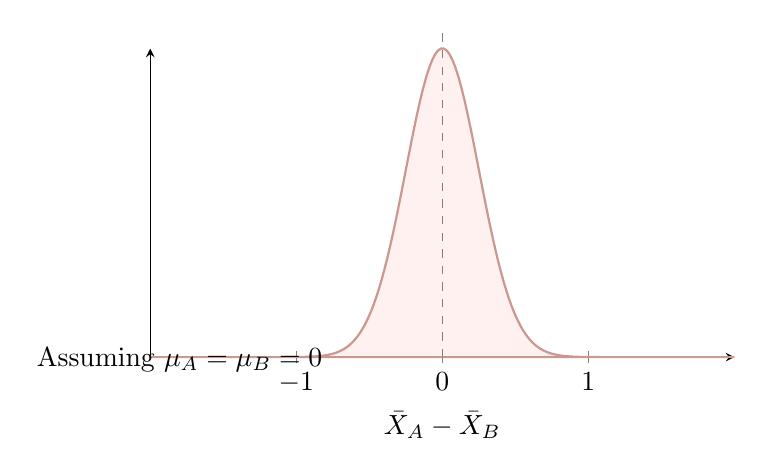
\begin{tikzpicture}
\begin{axis}[
  width=9cm, height=5.5cm,
  domain=-2:2,
  samples=200,
  axis lines=left,
  xlabel={$\bar{X}_A - \bar{X}_B$},
  ylabel={},
  xtick={-1, 0, 1},
  xticklabels={$-1$, $0$, $1$},
  ytick=\empty,
  clip=false
]
  % Normal curve centered at 0 with std = 1/4
  \addplot[thick, softpink!80!black, fill=softpink!40, fill opacity=0.5]
    {exp(-((x)^2)/(2*(0.25)^2)) / (0.25*sqrt(2*pi))}
    \closedcycle;
  % Shade left tail (< -1)
  \addplot[fill=babyblue!60, fill opacity=0.7, draw=none, domain=-2:-1, samples=50]
    {exp(-((x)^2)/(2*(0.25)^2)) / (0.25*sqrt(2*pi))} \closedcycle;
  % Shade right tail (> 1)
  \addplot[fill=babyblue!60, fill opacity=0.7, draw=none, domain=1:2, samples=50]
    {exp(-((x)^2)/(2*(0.25)^2)) / (0.25*sqrt(2*pi))} \closedcycle;
  \draw[dashed, gray] (axis cs:0,0) -- (axis cs:0,1.7);
  \node[below] at (axis cs:-1.8, 0.1) {Assuming $\mu_A = \mu_B = 0$};
\end{axis}
\end{tikzpicture}
\end{center}

\textbf{Calculation.}
\begin{align*}
&P\!\left(\bar{X}_A - \bar{X}_B > 1 \;\Big|\; \mu_A = \mu_B\right) + P\!\left(\bar{X}_A - \bar{X}_B < -1 \;\Big|\; \mu_A = \mu_B\right) \\
&= 2\,P\!\left(\frac{(\bar{X}_A - \bar{X}_B) - 0}{1/4} > \frac{1 - 0}{1/4}\right)
= 2\,P(Z > 4) < 0.0001.
\end{align*}

\textbf{Conclusion.} The probability of observing a difference as large as 1 hour (in absolute value) under the null hypothesis is less than 0.0001. This is far below any reasonable significance level. We \textbf{reject} $\mu_A = \mu_B$ and conclude there is strong evidence of a difference in mean drying times.

\bigskip

% ============================================================
\section{Practice Problems}
% ============================================================

\begin{hwbox}[Practice 8.1 --- CLT: Sum of Random Variables (adapted from 2014 exam)]
\textbf{Problem.} Suppose that $X_1, \ldots, X_{200}$ are independent continuous random variables with common density function
\[
f(x) = 2(1-x) \quad \text{for } 0 \leq x \leq 1, \quad 0 \text{ otherwise.}
\]
Define $S = X_1 + \cdots + X_{200}$.

\begin{enumerate}[label=(\alph*)]
  \item Compute the mean and variance of $X_i$.
  \item Using an appropriate method, find an approximation for $P(S > 70)$.
  \item Now define $Y_i = 1$ if $X_i > 0.9$ and $Y_i = 0$ otherwise. Set $T = Y_1 + \cdots + Y_{200}$. Compute $P(T \geq 3)$.
\end{enumerate}

\textbf{Solution.}

(a) 
\[
E(X) = \int_0^1 x \cdot 2(1-x)\,dx = 2\int_0^1 (x - x^2)\,dx = 2\left[\frac{1}{2} - \frac{1}{3}\right] = \frac{1}{3}.
\]
\[
E(X^2) = \int_0^1 x^2 \cdot 2(1-x)\,dx = 2\left[\frac{1}{3} - \frac{1}{4}\right] = \frac{1}{6}.
\]
\[
\text{Var}(X) = E(X^2) - [E(X)]^2 = \frac{1}{6} - \frac{1}{9} = \frac{1}{18}.
\]

(b) By the CLT, $S$ is approximately normal with:
\[
E(S) = 200 \times \frac{1}{3} = \frac{200}{3} \approx 66.67, \qquad
\text{Var}(S) = 200 \times \frac{1}{18} = \frac{200}{18} \approx 11.11.
\]
\[
P(S > 70) = P\!\left(Z > \frac{70 - 200/3}{\sqrt{200/18}}\right) = P\!\left(Z > \frac{70 - 66.67}{\sqrt{11.11}}\right) = P(Z > 1.00) \approx 0.1587.
\]

(c) First, find $P(X_i > 0.9)$:
\[
P(X_i > 0.9) = \int_{0.9}^{1} 2(1-x)\,dx = \left[-(1-x)^2\right]_{0.9}^{1} = 0 - (-(0.1)^2) = 0.01.
\]
So $T = \sum_{i=1}^{200} Y_i \sim \text{Bin}(200,\; 0.01)$.

Exact computation:
\begin{align*}
P(T \geq 3) &= 1 - P(T = 0) - P(T = 1) - P(T = 2) \\
&= 1 - \binom{200}{0}(0.01)^0(0.99)^{200} - \binom{200}{1}(0.01)^1(0.99)^{199} - \binom{200}{2}(0.01)^2(0.99)^{198} \\
&\approx 1 - 0.1340 - 0.2707 - 0.2720 = \boxed{0.3233.}
\end{align*}
\end{hwbox}

\begin{hwbox}[Practice 8.2 --- Hypothesis Test on Population Mean (adapted from 2015 exam)]
\textbf{Problem.} A program was run 6 times with randomly chosen data sets. The sample mean and sample standard deviation of execution times were $\bar{x} = 228$ ms and $s = 14$ ms, respectively.

\begin{enumerate}[label=(\alph*)]
  \item Compute a 95\% confidence interval for the true mean execution time. State your assumptions.
  \item It is claimed that the overall mean execution time is less than 230 ms. Do the data support this claim? Use $\alpha = 0.05$.
\end{enumerate}

\textbf{Solution.}

(a) The sample is small ($n = 6$) and $\sigma$ is unknown, so we assume the population is normally distributed and use the $t$-distribution with $n-1 = 5$ degrees of freedom.

$t_{5;\, 0.025} = 2.571$. The 95\% CI is:
\[
\bar{x} \pm t_{n-1;\, \alpha/2}\,\frac{s}{\sqrt{n}} = 228 \pm 2.571 \times \frac{14}{\sqrt{6}} = 228 \pm 14.7 = (213.3,\; 242.7)\,\text{ms.}
\]

(b) Hypotheses: $H_0{:}\; \mu = 230$ vs.\ $H_a{:}\; \mu < 230$.
\[
t_{\text{stat}} = \frac{\bar{x} - \mu_0}{s/\sqrt{n}} = \frac{228 - 230}{14/\sqrt{6}} = -0.35.
\]
The critical value is $-t_{5;\, 0.05} = -2.015$. Since $t_{\text{stat}} = -0.35 > -2.015$, we \textbf{fail to reject} $H_0$. The data do not provide sufficient evidence to support the claim.
\end{hwbox}

\begin{hwbox}[Practice 8.3 --- Two-Sample Inference on Means (adapted from 2015 exam)]
\textbf{Problem.} A company supporting two types of computer networks measures downtime (hours/year):

\begin{center}
\begin{tabular}{lcc}
\hline
 & Type 1 & Type 2 \\
\hline
Sample size & 10 & 9 \\
Sample mean & 83.5 & 60.4 \\
Standard deviation & 34.2 & 22.3 \\
\hline
\end{tabular}
\end{center}

\begin{enumerate}[label=(\alph*)]
  \item Test whether the two populations have different variances at $\alpha = 0.10$.
  \item Assuming equal variances, is there a significant difference in mean downtime? Use $\alpha = 0.10$.
\end{enumerate}

\textbf{Solution.}

(a) $H_0{:}\; \sigma_1^2 = \sigma_2^2$ vs.\ $H_a{:}\; \sigma_1^2 \neq \sigma_2^2$.
\[
F_{\text{stat}} = \frac{s_1^2}{s_2^2} = \frac{34.2^2}{22.3^2} = \frac{1169.64}{497.29} \approx 2.352.
\]
Critical value: $F_{(9,8);\, 0.05} = 3.39$. Since $2.352 < 3.39$, we \textbf{fail to reject} $H_0$. There is no significant evidence of unequal variances.

(b) Using the pooled $t$-test (equal variance assumed):
\[
s_p^2 = \frac{(n_1-1)s_1^2 + (n_2-1)s_2^2}{n_1+n_2-2} = \frac{9 \times 34.2^2 + 8 \times 22.3^2}{17} \approx 853.24.
\]
$t_{17;\, 0.05} = 1.740$. The 90\% CI for $\mu_1 - \mu_2$:
\[
(83.5 - 60.4) \pm 1.740\sqrt{853.24\left(\frac{1}{10}+\frac{1}{9}\right)} = 23.1 \pm 22.85 \approx (0.25,\; 45.95).
\]
Since the CI does not contain 0, we \textbf{reject} $H_0$ at $\alpha = 0.10$ and conclude there is a significant difference in mean downtime.
\end{hwbox}

\begin{hwbox}[Practice 8.4 --- Inference and Power (adapted from 2015 exam)]
\textbf{Problem.} Define $X_1, \ldots, X_{100}$ to be independent Normal r.v.'s with unknown mean $\mu$ and variance 25. Test $H_0{:}\; \mu = 10$ vs.\ $H_1{:}\; \mu \neq 10$ using test statistic $\bar{X} = \frac{1}{100}\sum_{i=1}^{100} X_i$. Reject $H_0$ if $\bar{X} \geq 10.98$ or $\bar{X} \leq 9.02$.

\begin{enumerate}[label=(\alph*)]
  \item Find the significance level of the test.
  \item If the true value is $\mu = 10.5$, find the power of the test.
\end{enumerate}

\textbf{Solution.}

(a) Under $H_0$, $\bar{X} \sim N\!\left(10,\, \frac{25}{100}\right) = N(10, 0.25)$, so $\text{SD}(\bar{X}) = 0.5$.
\[
\alpha = P(\bar{X} \geq 10.98) + P(\bar{X} \leq 9.02) = 2\,P\!\left(Z > \frac{10.98-10}{0.5}\right) = 2\,P(Z > 1.96) = 2(0.025) = \boxed{0.05.}
\]

(b) Under $H_1\colon \mu = 10.5$, $\bar{X} \sim N(10.5, 0.25)$.
\begin{align*}
\text{Power} &= P(\bar{X} \geq 10.98 \mid \mu=10.5) + P(\bar{X} \leq 9.02 \mid \mu=10.5) \\
&= P\!\left(Z > \frac{10.98 - 10.5}{0.5}\right) + P\!\left(Z < \frac{9.02 - 10.5}{0.5}\right) \\
&= P(Z > 0.96) + P(Z < -2.96) \\
&\approx 0.1685 + 0.0015 = \boxed{0.17.}
\end{align*}
\end{hwbox}

\begin{hwbox}[Practice 8.5 --- Sampling Distribution of Difference (two paints)]
\textbf{Problem.} Suppose specimens are painted with Paint A or Paint B. We know $\sigma_A = \sigma_B = 1$ hour, and independent samples of size $n_A = n_B = 32$ are taken. The observed difference is $\bar{x}_A - \bar{x}_B = 1$.

\begin{enumerate}[label=(\alph*)]
  \item State the null and alternative hypotheses for testing whether the paints differ in mean drying time.
  \item Under $H_0$, what is the sampling distribution of $\bar{X}_A - \bar{X}_B$?
  \item Compute the $p$-value and state your conclusion.
\end{enumerate}

\textbf{Solution.}

(a) $H_0{:}\; \mu_A = \mu_B$ (equivalently $\mu_A - \mu_B = 0$) vs.\ $H_a{:}\; \mu_A \neq \mu_B$.

(b) Under $H_0$:
\[
\bar{X}_A - \bar{X}_B \sim N\!\left(0,\; \frac{1}{32} + \frac{1}{32}\right) = N\!\left(0,\; \frac{1}{16}\right),
\quad \text{SD} = \frac{1}{4}.
\]

(c)
\[
p\text{-value} = 2\,P\!\left(\bar{X}_A - \bar{X}_B > 1\right) = 2\,P\!\left(Z > \frac{1 - 0}{1/4}\right) = 2\,P(Z > 4) < 0.0001.
\]
Since $p < 0.05$, we \textbf{reject} $H_0$ and conclude that the paints have different mean drying times.
\end{hwbox}

\begin{hwbox}[Practice 8.6 --- Hypothesis Test: Binomial with Normal Approximation (adapted from 2014 exam)]
\textbf{Problem.} Suppose that $X$ is a Binomial random variable with $n = 100$ and unknown $p$. We want to test $H_0{:}\; p = 0.4$ against $H_1{:}\; p > 0.4$. We reject $H_0$ if $X \geq 48$. Use normal approximations throughout.

\begin{enumerate}[label=(\alph*)]
  \item Find the significance level ($\alpha$) for this test.
  \item Suppose that the true value of $p$ is 0.55. Find the power of the test.
\end{enumerate}

\textbf{Solution.}

(a) Under $H_0$, $X \sim \text{Bin}(100, 0.4)$, so $\mu = 40$, $\sigma = \sqrt{100 \times 0.4 \times 0.6} = \sqrt{24}$.
\[
\alpha = P(X \geq 48 \mid p = 0.4) \approx P\!\left(Z \geq \frac{47.5 - 40}{\sqrt{24}}\right) = P\!\left(Z \geq \frac{7.5}{4.899}\right) = P(Z \geq 1.531) \approx \boxed{0.063.}
\]

(b) Under $H_1$, $X \sim \text{Bin}(100, 0.55)$, so $\mu = 55$, $\sigma = \sqrt{100 \times 0.55 \times 0.45} = \sqrt{24.75}$.
\[
\text{Power} = P(X \geq 48 \mid p = 0.55) \approx P\!\left(Z \geq \frac{47.5 - 55}{\sqrt{24.75}}\right) = P\!\left(Z \geq \frac{-7.5}{4.975}\right) = P(Z \geq -1.508) \approx \boxed{0.934.}
\]
\end{hwbox}

\begin{hwbox}[Practice 8.7 --- Assessing Normality (adapted from 2013 exam)]
\textbf{Problem.} A machine produces metal rods. A random sample of 21 rods is selected and the diameter of each is measured. Assuming normality, a 95\% confidence interval was constructed.

\begin{enumerate}[label=(\alph*)]
  \item How might you assess the assumption of normality? State two different methods. For each, indicate what would suggest normality and what would suggest non-normality.
\end{enumerate}

\textbf{Solution.}

\begin{enumerate}[label=(\alph*)]
  \item Two methods to assess normality:
  
  \textbf{Method 1: Normal QQ-plot (or normal probability plot).} Plot the data quantiles against the theoretical normal quantiles. If the points fall approximately on a straight line, this supports the normality assumption. Systematic curvature or deviations from linearity suggest non-normality.
  
  \textbf{Method 2: Formal hypothesis test} (e.g., Shapiro--Wilk test, chi-squared goodness-of-fit test). If you reject the null hypothesis (that the data come from a normal distribution), there is evidence of non-normality. If you fail to reject, the normality assumption is not contradicted.
\end{enumerate}
\end{hwbox}

\begin{hwbox}[Practice 8.8 --- Sample Size for Power (adapted from 2013 exam)]
\textbf{Problem.} Suppose $X_1, \ldots, X_n$ are i.i.d.\ $N(\mu, 1)$. We test $H_0{:}\; \mu = 10$ vs.\ $H_a{:}\; \mu \neq 10$ at the 5\% level, rejecting if $\bar{X} > 10 + 1.96/\sqrt{n}$ or $\bar{X} < 10 - 1.96/\sqrt{n}$. If the true value of $\mu$ is 10.1, how large must $n$ be for the test to have power at least 0.90?

\textbf{Solution.}

Under $H_a\colon \mu = 10.1$:
\begin{align*}
\text{Power} &= P\!\left(\bar{X} > 10 + \frac{1.96}{\sqrt{n}} \;\Big|\; \mu = 10.1\right) + P\!\left(\bar{X} < 10 - \frac{1.96}{\sqrt{n}} \;\Big|\; \mu = 10.1\right).
\end{align*}

The second term approaches 0 quickly. Focusing on the dominant term:
\[
P\!\left(Z > \frac{10 + 1.96/\sqrt{n} - 10.1}{1/\sqrt{n}}\right) = P\!\left(Z > 1.96 - 0.1\sqrt{n}\right) \geq 0.90.
\]

For $P(Z > c) = 0.90$, we need $c = -1.28$ (approximately). So:
\[
1.96 - 0.1\sqrt{n} = -1.28 \implies 0.1\sqrt{n} = 3.24 \implies \sqrt{n} = 32.4 \implies n \approx 1050.
\]

Therefore, $n$ must be at least approximately $\boxed{1050}$ (the exact answer with full normal probabilities is $n = 1051$).
\end{hwbox}

\end{document}
